\newpage
\section{Gestione amministrativa della revisione}
\subsection{Comunicazione delle anomalie}
Il \glossaryItem{processo} di Software Quality Management è finalizzato alla ricerca dei difetti. L'identificazione delle \glossaryItem{anomalie} mantiene aggiornato il Responsabile sullo stato del prodotto, e permette di prendere dei provvedimenti per correggerle. A tal fine, è utile distinguere e catalogare le \glossaryItem{anomalie}, per discuterne durante revisioni e riunioni. Il \glossaryItem{team} ha scelto di adottare le definizioni di \glossaryItem{anomalie} presenti nello standard IEEE 610.12-90:
\begin{itemize}
\item \textbf{Error}: differenza tra un valore (o una condizione) calcolato, osservato o misurato e il vero, specifico, corretto valore (o condizione). Gli errori sono stati interni di un sistema che, infine, si manifestano nel suo comportamento esterno. La causa di un errore si indica con il termine fault;
\item \textbf{Fault}: passo, \glossaryItem{processo} o dato definito in modo erroneo (e.g. violazioni delle norme tipografiche di un documento). \`E anche noto con il nome di bug.
\item \textbf{Failure}: la conseguenza di un fault (e.g. incongruenza del prodotto rispetto alle funzionalità indicate nell'analisi dei requisiti);
\item \textbf{Mistake}: azione umana che produce un risultato errato.
\end{itemize}
Questa catalogazione permette di definire delle metriche in grado di valutare l'andamento del prodotto e, in alcuni casi, di predirlo. Un esempio è la metrica che conteggia il numero di bug per linee di codice.

\subsection{Controlli per la qualità di processo}
Le procedure di controllo per la \glossaryItem{qualità} di \glossaryItem{processo} sono finalizzate a migliorare la \glossaryItem{qualità} del prodotto e/o diminuire i costi e tempi di sviluppo. Esistono due approcci principali:
\begin{itemize}
\item \textbf{A maturità di \glossaryItem{processo}}: l'obiettivo primario è la \glossaryItem{qualità} del prodotto e la prevedibilità dei processi;
\item \textbf{Agile}: sviluppo iterativo senza l'\glossaryItem{overhead} della documentazione e di tutti gli aspetti predeterminabili. Ha come caratteristica la \glossaryItem{responsività} ai cambiamenti dei requisti cliente e uno sviluppo rapido.
\end{itemize}
Il primo approccio è maggiormente indicato ad un \glossaryItem{team} con poca esperienza: verrà pertanto scelto quello. Con una visione \glossaryItem{proattiva} si cerca di avere maggior controllo e previsione sulle attività da svolgere. Questa viene anche indicata come best practice per gruppi poco esperti.\\
Il \glossaryItem{processo} con maggiore influenza sulla \glossaryItem{qualità} del sistema non è quello di sviluppo ma quello di progettazione. È qui che le capacità e le esperienze dei singoli danno un contributo decisivo.\\
\begin{figure}[h]
\centering 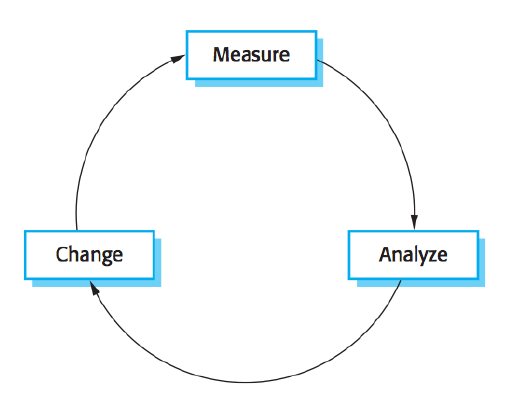
\includegraphics[width=0.8\textwidth]{res/sections/processImprovement.png}
\caption{Il ciclo di miglioramento dei processi}
\end{figure}
Il miglioramento dei processi è un \glossaryItem{processo} ciclico, composto da tre sotto-processi:
\begin{itemize}
\item \textbf{Misurazione del \glossaryItem{processo}}: misura gli attributi del \glossaryItem{progetto}, punta ad allineare gli obiettivi con le misurazioni effettuate. Questo forma una baseline che aiuta a capire se i miglioramenti hanno avuto effetto;
\item \textbf{Analisi del \glossaryItem{processo}}: vengono identificate le problematiche ed i colli di bottiglia dei processi;
\item \textbf{Modifiche del \glossaryItem{processo}}: i cambiamenti vengono proposti in risposta alle problematiche riscontrate.
\end{itemize}
Il \glossaryItem{team} procederà nel seguente modo: 
\begin{itemize}
\item Nella sezione \textit{Dettaglio delle verifiche tramite analisi} (\ref{App:AppendixB})  verranno inserite le misurazioni rilevate sulle le metriche descritte in \textit{Misure e Metriche} (\ref{MisureMetriche});
\item L'analisi viene effettuata i giorni precedenti alle consegne previste dal \glossaryItem{committente}; il \textit{Riassunto delle attività di \glossaryItem{verifica}} (\ref{App:AppendixA}) contiene l'analisi del \glossaryItem{processo}, le relative considerazioni  comprendenti le problematiche riscontrate;
\item Le modifiche al \glossaryItem{processo} vengono attuate all'inizio del \glossaryItem{processo} incrementale successivo. Queste attività sono programmate nel \PianoDiProgetto.
\end{itemize}
